% Citation dummy
We will probably cite~\cite{goeltz2020fast} in line with the figures~\cref{fig:setup,fig:setupwithtikz} as they originate from said paper.
Furthermore, an example use of a glossary entry with \gls{snn}.

\lipsum[2]


\begin{figure}
  \centering
  \includegraphics[width=0.48\textwidth]{../../fig/figSetup.pdf}
  \caption{
      once without tikz
  }\label{fig:setup}
\end{figure}



\begin{figure}
  \centering
  \includegraphics[width=0.48\textwidth]{../tikz/figSetup/figSetup.pdf}
  \caption{
      and once with tikz graphs
  }\label{fig:setupwithtikz}
\end{figure}
